\chapter{Versuch 1}
\label{chap:VERSUCH_1}

\section{Fragestellung, Messprinzip, Aufbau, Messmittel}
\label{chap:VERSUCH_1_FRAGESTELLUNG}

Bei Versuch 1 ging es um die Messung von Abständen mittels eines Entfernungssensors.

\subsection*{Fragestellung}

	Sinn: Abstände mittels Sensor messen um dann Fehler zu ermitteln
\subsection*{Messprinzip}

	Triangulationsprinziep
	füge das Bild aus Anleitung ein
\subsection*{Aufbau}
	hier screenshot einfügen und beschriften. Das Bild an die richtige stelle zu bekommen ist knifflig, wir sollten lieber schauen, das die Bildunterschrift stimmt.
	\begin{figure}[h] % [hbtp] einstellungsoptionen für bilder, sind aber nicht empfohlen
		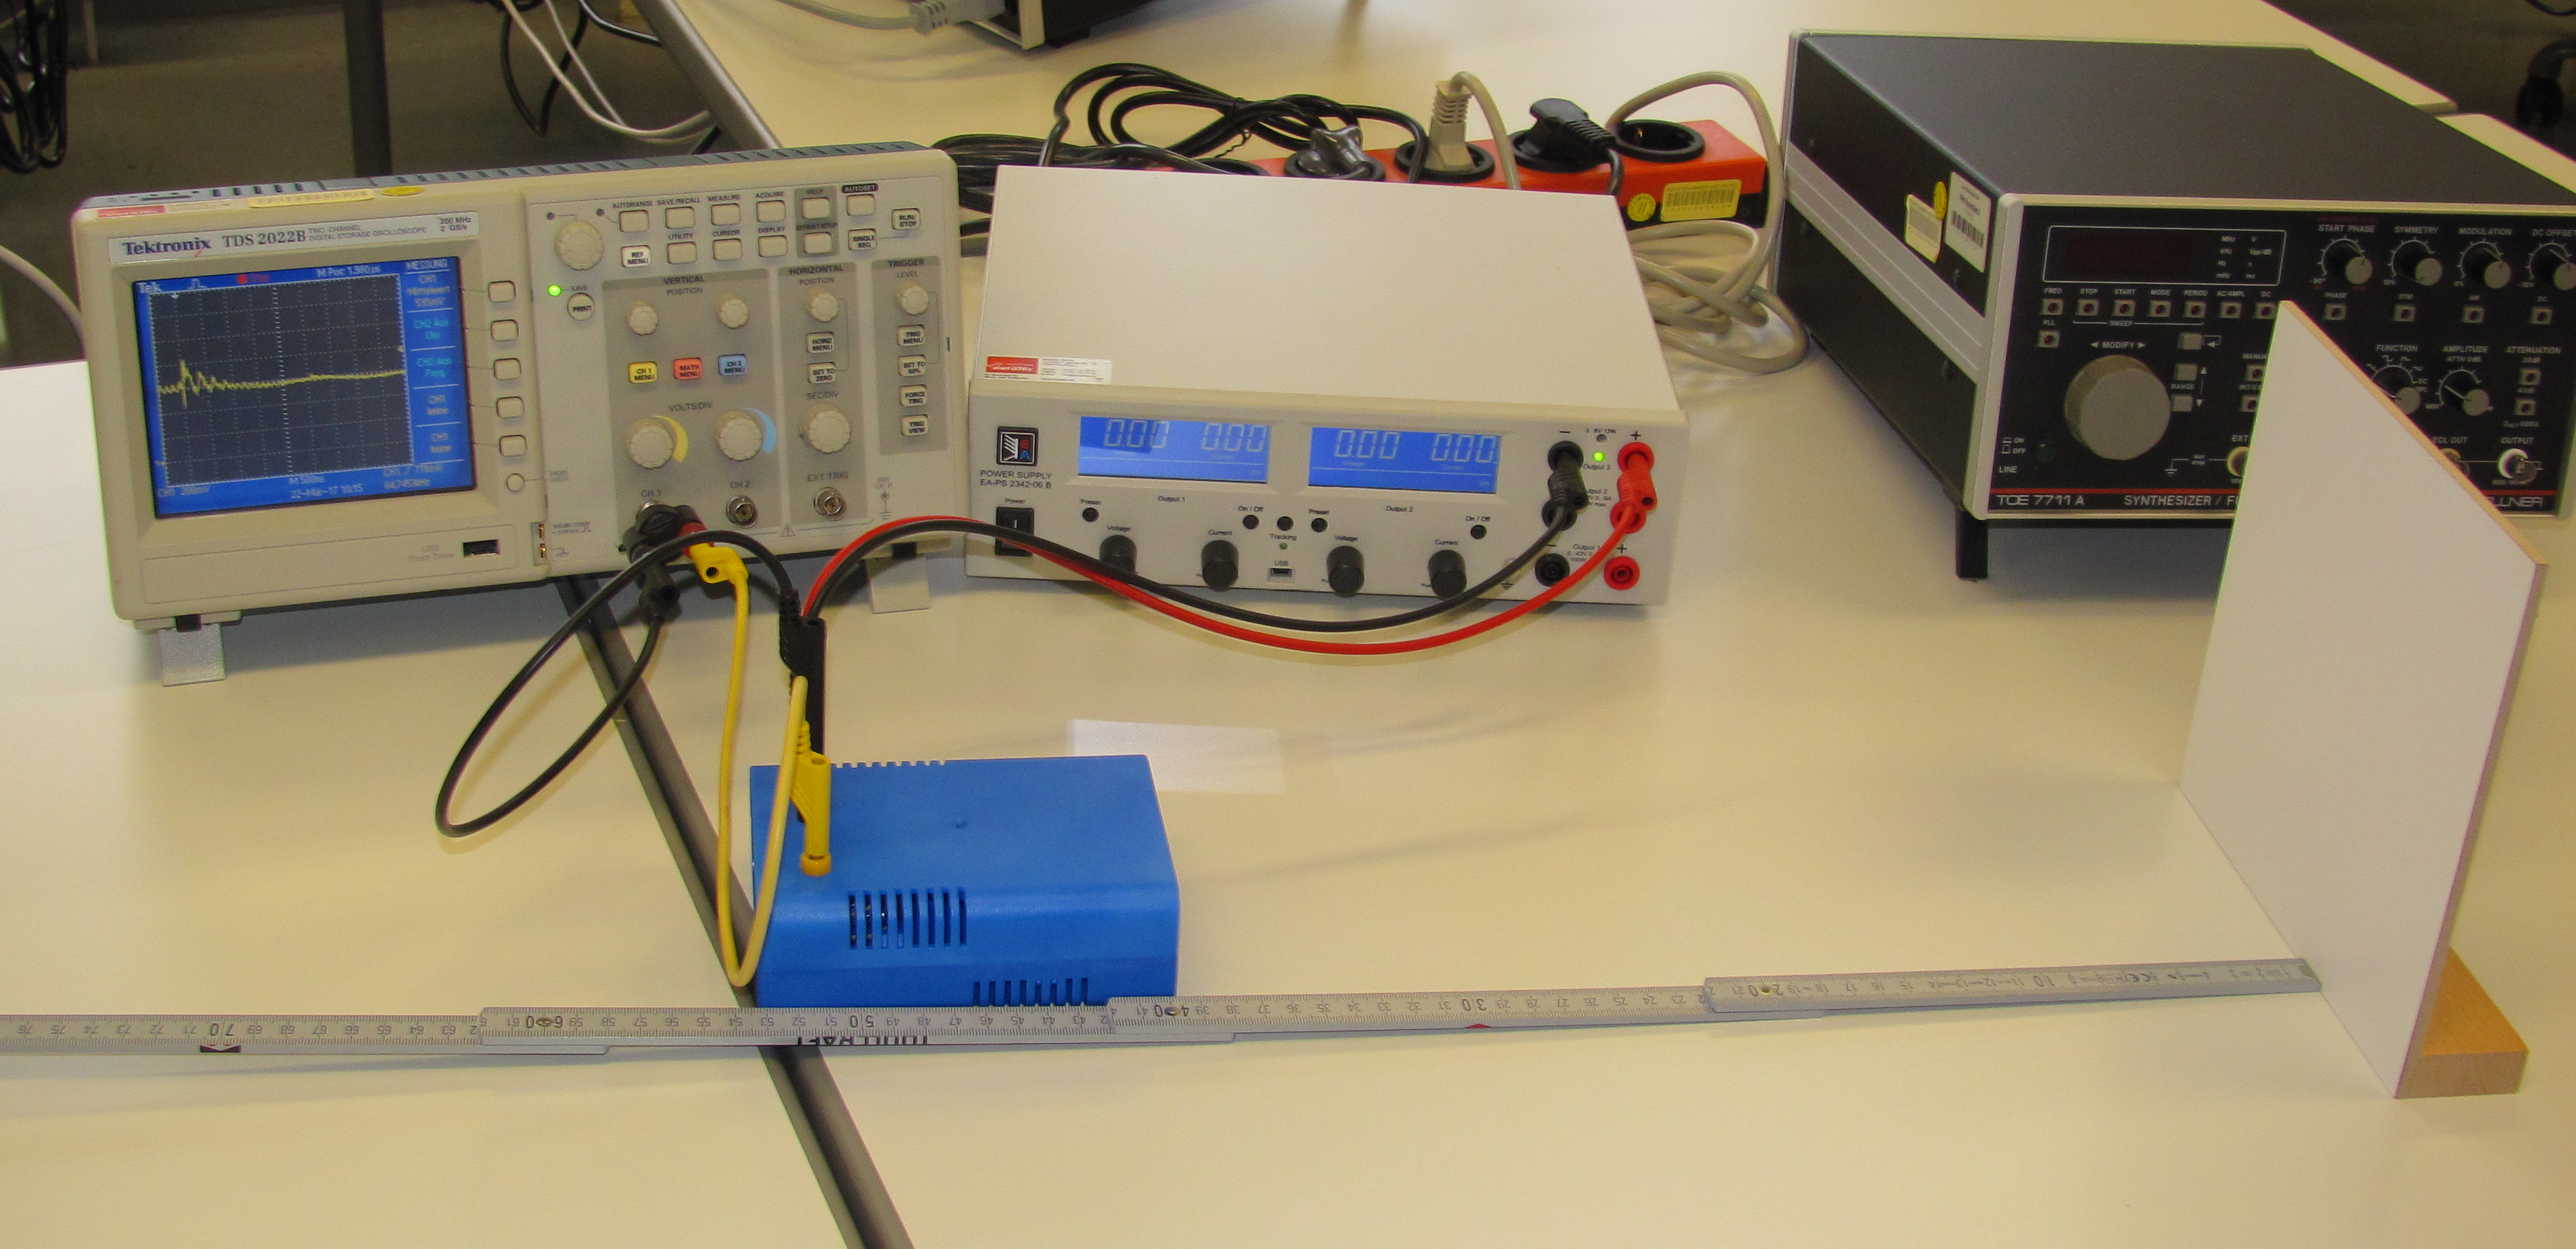
\includegraphics[scale=0.15]{media/aufbau.png}
		\label{Versuchsaufbau}
	\end{figure}

\subsection*{Messmittel}
	zur Messung wurden folgende Messmittel benutzt:
	\begin{itemize}
		\item Sensor(Abstandmessungssensor)
		\item Osziloskop
		\item Metermaß
		\item Brett (als Objekt dessen abstand gemessen wird)
	\end{itemize}


\section{Messwerte}
\label{chap:VERSUCH_1_MESSWERTE}

\section{Auswertung}
\label{chap:VERSUCH_1_AUSWERTUNG}


\section{Interpretation}
\label{chap:VERSUCH_1_INTERPRETATION}
